% !TeX program = lualatex
\documentclass[../skript/main.tex]{subfiles}

\begin{document}
\chapter{Zahlensysteme}\label{chap:zahlensysteme}

\section{Was ist ein Zahlensystem?}
Ein \textbf{Zahlensystem} legt fest, wie Zahlen durch \emph{Ziffern} und deren \emph{Stellenwert} dargestellt werden.
In \emph{Stellenwertsystemen} (positionalen Systemen) hat jede Stelle einen Wert, der von der \emph{Basis} \(b\) abhängt:
\[
(d_k d_{k-1}\ldots d_1 d_0)_b
= d_k\cdot b^{k}+d_{k-1}\cdot b^{k-1}+\ldots + d_1\cdot b^1 + d_0\cdot b^0,
\]
wobei \(0 \le d_i < b\) gilt. Beispiele: Dezimal (\(b=10\)), Binär (\(b=2\)), Oktal (\(b=8\)), Hexadezimal (\(b=16\)).
Nicht-positionale Systeme (z.\,B. römische Zahlen) kennen keinen einheitlichen Stellenwert und sind für Rechenalgorithmen unpraktisch.

\section{Dezimalsystem (\(b=10\))}
Das \textbf{Dezimalsystem} nutzt die Ziffern \(0\)–\(9\).
Es ist heute \emph{weltweit das dominante System für den Alltag und das schulische Rechnen}.
Historisch hängt das vermutlich mit dem Zählen an zehn Fingern zusammen.
Beispiel:
\[
(5073)_{10} = 5\cdot 10^3 + 0\cdot 10^2 + 7\cdot 10^1 + 3\cdot 10^0.
\]

\section{Andere Zahlensysteme in der Welt}
\subsection*{Sexagesimalsystem (\(b=60\))}
Das \textbf{Babylonische Sexagesimalsystem} prägt uns bis heute: \emph{Zeitmessung} (60\,s \(=\) 1\,min, 60\,min \(=\) 1\,h) und \emph{Winkelmaße} (Grad–Bogenmaß mit Minuten und Sekunden). Rechnen erfolgt im Alltag dennoch meist dezimal; die Einteilung selbst ist aber sexagesimal.

\subsection*{Vigesimalsystem (\(b=20\))}
In Teilen der Welt gab und gibt es \textbf{Zwanzigersysteme} (Basis 20).
Sprachliche Spuren finden sich z.\,B. in Zahlwörtern einiger Sprachen (Restbestände wie „vier-mal-zwanzig“ für 80).
Auch hier wird formal in der Schule und in modernen Anwendungen überwiegend dezimal gerechnet.

\subsection*{Duodezimalsystem (\(b=12\))}
Das \textbf{Zwölfersystem} hat gute Teilbarkeit (2,3,4,6). Reste davon sieht man bei Dutzend/Groß, Uhren (12 Stunden), Maßeinheiten aus der Geschichte. Für maschinelles oder schulisches Rechnen dominiert aber 10.

\subsection*{Fazit zur Frage: „Rechnet man irgendwo ernsthaft nicht-dezimal?“}
\textbf{Menschen} rechnen heute fast überall \emph{dezimal}, mit kulturellen Resten anderer Basen in speziellen Domänen (Zeit, Winkel, Maße).  
\textbf{Maschinen} (Computer) \emph{rechnen binär}. Darauf basiert die Notwendigkeit weiterer Basen in der Informatik (Oktal/Hex als kompakte Binärdarstellung).

\section{Binär, Oktal, Hexadezimal – warum in der Informatik?}
\subsection*{Binärsystem (\(b=2\))}
Digitale Schaltungen kennen zwei stabile Zustände (z.\,B. „aus“/„ein“). Deshalb arbeitet Hardware \emph{binär}.
\[
(101010)_2 = 1\cdot 2^5 + 0\cdot 2^4 + 1\cdot 2^3 + 0\cdot 2^2 + 1\cdot 2^1 + 0\cdot 2^0 = 42.
\]

\subsection*{Oktalsystem (\(b=8\)) und Hexadezimalsystem (\(b=16\))}
Beide sind für Menschen \emph{kompakte Schreibweisen} von Binärzahlen:
\begin{itemize}
	\item 1 \textbf{Oktal-Ziffer} entspricht \textbf{3 Bit} (weil \(8=2^3\)).
	\item 1 \textbf{Hex-Ziffer} entspricht \textbf{4 Bit} (weil \(16=2^4\)).
\end{itemize}
Darum lassen sich Binärzahlen leicht gruppieren:
\[
\underbrace{1010}_{\text{A}}\,\underbrace{1010}_{\text{A}} = (\text{AA})_{16} = (10101010)_2.
\]
Hex ist heute Standard in Programmierung, Speicher-Dumps, Farbwerten (\#FF00AA), Adressen usw.
Oktal sieht man u.\,a. noch bei UNIX-Rechten (z.\,B. \(0755\)).

\section{Umrechnungen zwischen Basen}
\subsection*{Von Dezimal in eine Basis \(b\) (Divisionsrest-Methode)}
Beispiel: \(93_{10}\) nach Binär.
\[
\begin{array}{r|l}
	93:2 = 46 \text{ Rest }1\\
	46:2 = 23 \text{ Rest }0\\
	23:2 = 11 \text{ Rest }1\\
	11:2 = 5  \text{ Rest }1\\
	5:2  = 2  \text{ Rest }1\\
	2:2  = 1  \text{ Rest }0\\
	1:2  = 0  \text{ Rest }1
\end{array}
\Rightarrow\ (93)_{10} = (1011101)_2.
\]

\subsection*{Von Basis \(b\) nach Dezimal (Horner-Schema)}
Beispiel: \((2A)_{16}\) mit \(A=10\):
\[
(2A)_{16} = 2\cdot 16^1 + 10\cdot 16^0 = 32 + 10 = 42.
\]

\subsection*{Direkt zwischen Binär, Oktal, Hex}
Gruppieren in 3er- bzw. 4er-Blöcke (von rechts):
\[
(110\ 010\ 111)_2 = (627)_8,\qquad
(1010\ 1111)_2 = (\text{AF})_{16}.
\]

\section{Beispiele}
\begin{center}
	\begin{tabular}{r|c|c|c}
		\textbf{Dezimal} & \textbf{Binär} & \textbf{Oktal} & \textbf{Hex} \\
		\hline
		10 & \(1010\) & \(12\) & A \\
		26 & \(11010\) & \(32\) & 1A \\
		42 & \(101010\) & \(52\) & 2A \\
		64 & \(1000000\) & \(100\) & 40 \\
		100 & \(1100100\) & \(144\) & 64 \\
	\end{tabular}
\end{center}

\section{Die Zweierkomplementdarstellung}

\subsection{Worum geht es?}
Computer speichern Zahlen als Bitmuster. Für \emph{positive} ganze Zahlen ist das einfach (normale Binärdarstellung). 
Aber wie speichern wir \emph{negative} Zahlen so, dass Addieren und Subtrahieren trotzdem mit der \emph{gleichen Hardware} funktionieren?
Die Antwort ist die \textbf{Zweierkomplementdarstellung}.

\subsection{Warum verwendet man das Zweierkomplement?}
\begin{itemize}
	\item \textbf{Ein Addierwerk für alles:} Dieselbe Schaltung addiert sowohl positive als auch negative Zahlen; Subtraktion wird als „Addiere das Zweierkomplement“ ausgeführt.
	\item \textbf{Eindeutige Null:} Es gibt nur \emph{eine} Null (anders als bei Vorzeichen-\&-Betrag oder Einerkomplement).
	\item \textbf{Einfache Regeln:} Vorzeichenverlängerung (Sign Extension) ist trivial: führende Einsen bei negativen Zahlen, Nullen bei positiven.
	\item \textbf{Sortier-/Vergleichsfreundlich:} Bei festem Wortbreite-Vergleich funktioniert das wie erwartet.
	\item \textbf{Mathematisch sauber:} Der Wertebereich ist genau \(-2^{n-1},\ldots,0,\ldots,2^{n-1}-1\) für \(n\)~Bit.
\end{itemize}

\begin{figure}[H]
	\centering
	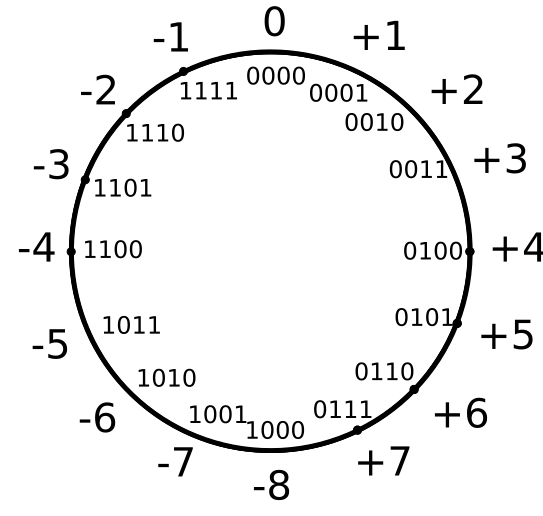
\includegraphics[width=.65\textwidth]{4Bit-2Komplement.png}
	\caption{4-Bit-Zweierkomplement: Zuordnung der Bitmuster zu Dezimalwerten und Bildung der negativen Werte (\(+1\) nach Bitinvertierung).}
	\label{fig:zweierkomplement-4bit}
\end{figure}

\subsection{So bildet man das Zweierkomplement (aus einer positiven Zahl \(x\))}
Für eine feste Wortbreite (z.\,B. 8~Bit):
\begin{enumerate}
	\item Schreibe \(x\) binär mit führenden Nullen.
	\item \textbf{Alle Bits invertieren} (0\,\(\leftrightarrow\)\,1).
	\item \textbf{+1 addieren.}
\end{enumerate}
Beispiel: \(-5\) als 8-Bit-Zahl. \\
\(+5 = \texttt{00000101}\ \Rightarrow\) invertiert \(\texttt{11111010}\ \Rightarrow\) \(+1\) \(\Rightarrow\) \(\boxed{\texttt{11111011}}\).

\subsection*{So liest man ein Zweierkomplement-Bitmuster}
\begin{itemize}
	\item \textbf{MSB (Most Significant Bit) = 0} \(\Rightarrow\) positive Zahl: normal als Binärzahl lesen.
	\item \textbf{MSB (Most Significant Bit) = 1} \(\Rightarrow\) negative Zahl: wieder positiv machen durch \emph{invertieren + 1} und ein Minus davor.
\end{itemize}
Beispiel: \(\texttt{11101100}\) (8~Bit) \(\Rightarrow\) invertieren \(\texttt{00010011}\), \(+1\) \(\Rightarrow\) \(\texttt{00010100} = 20\) \(\Rightarrow\) Wert ist \(-20\).

\subsection*{Wertebereich}
Für \(n\)~Bit gilt:
\[
\boxed{\ -2^{n-1}\ \le\ \text{Wert}\ \le\ 2^{n-1}-1\ }\quad
\text{(z.\,B. 4~Bit: \(-8\) bis \(+7\)).}
\]
Auffällig: Es gibt \emph{kein} \(+2^{n-1}\) (bei 4~Bit also kein \(+8\)); das Muster \(\texttt{1000}\) steht für \(-8\).

\subsection*{Rechnen mit Zweierkomplement}
\paragraph{Addition/Subtraktion.}
\begin{itemize}
	\item Subtraktion \(a-b\) wird als \(a + (\text{Zweierkomplement von } b)\) gerechnet.
	\item \emph{Beispiel (4~Bit):} \(7 + (-3)\): \(\texttt{0111} + \texttt{1101} = \texttt{1 0100}\) \(\Rightarrow\) \(\texttt{0100} = 4\) (Übertrag links fällt weg).
\end{itemize}

\paragraph{Überlauf (Overflow) erkennen.}
\begin{itemize}
	\item \textbf{Regel:} Addiert man zwei \emph{positive} Zahlen und erhält eine \emph{negative}, oder zwei \emph{negative} und erhält eine \emph{positive}, dann ist Overflow aufgetreten.
	\item Alternativ technisch: Overflow, wenn \emph{Carry in} das Vorzeichenbit \(\neq\) \emph{Carry out} des Vorzeichenbits.
\end{itemize}

\paragraph{Vorzeichenverlängerung (Sign Extension).}
Erweitere eine Zweierkomplementzahl auf mehr Bit, indem du die \emph{linke führende Ziffer} wiederholst:
\begin{itemize}
	\item positiv: \(\texttt{0}\)en voran (z.\,B. \(\texttt{0010}\ \to\ \texttt{0000 0010}\))
	\item negativ: \(\texttt{1}\)en voran (z.\,B. \(\texttt{1110}\ \to\ \texttt{1111 1110}\))
\end{itemize}

\subsection*{Vergleich zu anderen Darstellungen}
\begin{description}
	\item[Vorzeichen \& Betrag:] Einfach zu verstehen (ein Bit fürs Vorzeichen), aber zwei Nullen (\(+0\) und \(-0\)) und Subtraktion ist umständlich.
	\item[Einerkomplement:] Auch zwei Nullen und kompliziertere Addition (End-Around-Carry).
	\item[Zweierkomplement:] \textbf{Standard in nahezu allen modernen CPUs} – schnell, eindeutig, hardwarefreundlich.
\end{description}

\subsection*{Beispiele (4-Bit)}
\begin{center}
	\begin{tabular}{c|r@{\qquad}c|r}
		\textbf{Bitmuster} & \textbf{Dezimal} & \textbf{Bitmuster} & \textbf{Dezimal} \\
		\hline
		\texttt{0111} & $+7$ & \texttt{1001} & $-7$ \\
		\texttt{0101} & $+5$ & \texttt{1011} & $-5$ \\
		\texttt{0000} & $0$  & \texttt{1111} & $-1$ \\
		\texttt{1000} & $-8$ & \texttt{1101} & $-3$ \\
	\end{tabular}
\end{center}

\section*{Wie rechnet ein Computer wirklich? — Ausblick}

Das Umwandeln von Zahlen und das schriftliche Rechnen zeigen \emph{wie} wir mit Binärzahlen umgehen. Ein Computer macht im Kern dasselbe — aber nicht „im Kopf“, sondern mit \textbf{logischen Operationen}, die in \textbf{elektronischen Schaltungen} realisiert sind. Grundlage ist die Boolesche Algebra: Aus einfachen Verknüpfungen wie \textsc{Nicht} (NOT), \textsc{Und} (AND), \textsc{Oder} (OR) und \textsc{Exklusiv-Oder} (XOR) werden Schaltungen aufgebaut, die Bits verarbeiten. Ein Addierer besteht beispielsweise aus \emph{Halb-} und \emph{Volladdierern}: Das \emph{Summenbit} entsteht über XOR (gerade/ungerade Anzahl von Einsen), der \emph{Übertrag} über AND/OR (Mehrheit der Einsen). Darum ist bei \(1+1\) das Summenbit \(0\) und der Übertrag \(1\) — genau wie in unseren schriftlichen Regeln.

Viele solcher Bausteine zusammen bilden die \textbf{ALU} (Arithmetic Logic Unit) einer CPU, gesteuert von einem \textbf{Takt}. \textbf{Register} und \textbf{Speicherzellen} (Flip-Flops) halten Zwischenwerte, und durch die feste Wortbreite rechnet die Hardware effektiv \(\bmod 2^n\) — daher kommen Phänomene wie \emph{Übertrag} und \emph{Overflow}. Auf höherer Ebene beschreibt \textbf{Software} die Abfolge dieser elementaren Operationen als Befehle und Algorithmen.

Mit diesen inneren Mechanismen — Logikgattern, Schaltnetzen und Schaltwerken, Transistoren und CMOS-Technik, aber auch endlichen Automaten — beschäftigen wir uns später im Kurs. Für jetzt reicht die Idee: Was wir schriftlich üben, setzt der Computer \emph{gleichbedeutend} durch logische Funktionen und Elektronik um.


\end{document}
